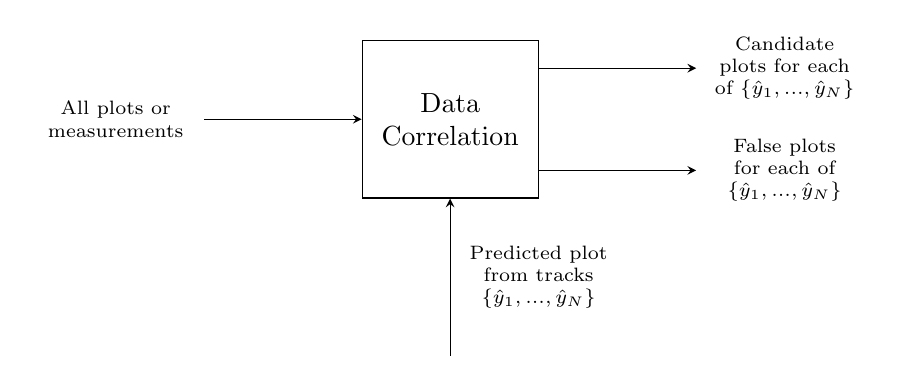
\begin{tikzpicture}[xscale=1,yscale=1,
	square/.style={rectangle, draw=black, text width=20mm, minimum height=20mm, align=center},
	label/.style={text width=20mm, align=center, font=\scriptsize},
	node distance= 2cm, >=stealth]
	
	%Nodes
	\node[square]	(dc)	at (0,0) {Data\\Correlation};
	
	%Lines
	\draw[black, <-] (dc.west) -- node [label, left, xshift=-10mm] {All plots or measurements} ++(-2,0);
	\draw[black, ->] (dc.30) -- node [label, right, xshift=10mm] {Candidate plots for each of $\{\hat{y}_1,...,\hat{y}_N\}$} ++(2,0);
	\draw[black, ->] (dc.330) -- node [label, right, xshift=10mm] {False plots for each of $\{\hat{y}_1,...,\hat{y}_N\}$} ++(2,0);
	\draw[black, <-] (dc.south) -- node [label, right] {Predicted plot from tracks $\{\hat{y}_1,...,\hat{y}_N\}$} ++(0,-2);
\end{tikzpicture}